\documentclass[10pt,twocolumn,letterpaper]{article}

\usepackage{cvpr}
\usepackage{times}
\usepackage{epsfig}
\usepackage{graphicx}
\usepackage{amsmath}
\usepackage{amssymb}
\usepackage{algorithm}

% Include other packages here, before hyperref.

% If you comment hyperref and then uncomment it, you should delete
% egpaper.aux before re-running latex.  (Or just hit 'q' on the first latex
% run, let it finish, and you should be clear).
\usepackage[breaklinks=true,bookmarks=false]{hyperref}

\cvprfinalcopy % *** Uncomment this line for the final submission

\def\cvprPaperID{****} % *** Enter the CVPR Paper ID here
\def\httilde{\mbox{\tt\raisebox{-.5ex}{\symbol{126}}}}

% Pages are numbered in submission mode, and unnumbered in camera-ready
%\ifcvprfinal\pagestyle{empty}\fi
\begin{document}

%%%%%%%%% TITLE
\title{TASE/P: Text-Audio Synchronization Engine and Platform}

\author{Arun Dunna\\
University of Massachusetts Amherst\\
Amherst, MA\\
{\tt\small adunna@cs.umass.edu}
% For a paper whose authors are all at the same institution,
% omit the following lines up until the closing ``}''.
% Additional authors and addresses can be added with ``\and'',
% just like the second author.
% To save space, use either the email address or home page, not both
}

\maketitle
%\thispagestyle{empty}

%%%%%%%%% ABSTRACT
\begin{abstract}
Bi-directional audio-text synchronization is both a problem of scale and of capabilities. Current systems, such as Amazon's WhisperSync\cite{} and LearningAlly\cite{}, use proprietary software that doesn't generalize and must run on large servers. Our solution, TASE, is an engine designed to synchronize words contained in a document or a collection of documents (for example, a PDF file) with speech found in an audio file or a collection of audio files. This engine is modular, allowing compatibility with other projects, such as TASP. In addition, we allow for synchronization that scales both up and down, allowing TASE to be used efficiently on large servers as well as on average consumer hardware. TASE leverages audio-to-text conversion models along with novel search methods, and several additional optimization features, to bring text-audio synchronization to the average consumer. This allows for a variety of implementations, such as prepared speech synchronization for the deaf, automatic validation of audio transcription services, or simple but convenient niceties such as listening to a book in the car and picking it back up in bed.
\end{abstract}

%%%%%%%%% BODY TEXT
\section{Introduction}
Text and audio are two of the largest mediums for information. From the news to textbooks to podcasts, we are constantly consuming information through reading and listening. Often times, we find ourselves wanting to bridge this gap. Specifically, we want to synchronize timestamps in audio with word positions in text. Perhaps the most common occurrence of this is listening to a book in your car, then finding yourself wanting to pick up where you left off on your eReader in bed.

Some platforms\cite{https://support.google.com/accessibility/android/answer/6283677?hl=en} offer text-to-speech (TTS) technologies to narrate your eBook. However, most TTS technologies today lack the emotions shown when reading a book aloud. Even the newest systems\cite{https://cloud.google.com/text-to-speech/} find it difficult to synthesize voices in the most realistic way possible. As a result, a few services exist to synchronize audiobooks with eBooks, such as Amazon's WhisperSync\cite{} which pairs Kindle\cite{} with Audible\cite{}, or LearningAlly\cite{}, which helps readers with disabilities. The caveat is that these platforms are both niche and closed-source, and are not easily scalable to other mediums such as lectures or speeches.

To solve this problem, we propose and develop the Text-Audio Synchronization Engine (TASE), and an example implementation in the Text-Audio Synchronization Platform (TASP). TASE is modular, allowing for developers to easily implement it in their own projects. It automatically scales, meaning that it can be implemented at the commercial level as a service, or can be run on a private instance for use by a small family. It relies on no third-party APIs, reducing the amount of data that flows to advertisers. Lastly, TASE can be extended to a variety of mediums by simply training on a different dataset; the synchronization method is exactly the same. Users can use TASE with a model trained on speeches with transcripts in order to synchronize the two with higher efficiency and accuracy.

\section{Background}
TODO

\section{Related Work}
Synchronization between audio and text by associating text fragments with audio timestamps in advance has been known for some time. Some projects attempt to do this automatically, such as aeneas\cite{https://www.readbeyond.it/aeneas/}. However, this requires a lot of upfront resources to analyze, and requires clear recordings as they rely on slicing based on pauses. Consumers typically do not have machines that can do these computations with hours of audio, and narrations often don't conform to the assumptions that these systems make.

As a result, we utilize machine learning to aid in the synchronization process through custom audio-to-text conversion models. As far as we are aware, this is an novel technique. The source for platforms such as WhisperSync and LearningAlly is not available, so it is not possible to compare, but based on the capabilities of these platforms it is a fair assumption.

\section{Methodology}
TODO.

For the rest of this paper, we refer to audio positions as timestamps, and text positions as word positions. Audio timestamps are recorded in milliseconds (ms).
\subsection{Audio to Text Conversion}
For our audio-to-text conversion, the main process that bridges the gap between the two mediums, we utilize Mozilla's implementation\cite{} of Baidu's DeepSpeech\cite{} model. This is implemented using Google's TensorFlow\cite{}, which allows for compatibility with both GPU and CPU processing, aiding with model performance at scale. Specifically, we use a bi-directional recurrent neural network (BDRNN) in which our input consists of features extracted directly from the audio (Figure~\ref{fig:model-arch}). We first pass our features through three fully connected (FC) layers with ReLU activation. These layers feed into a BDRNN layer, and the output characters from the BDRNN layer are then passed into the last FC layer, which uses LSTM with tanh activation\cite{https://hacks.mozilla.org/2017/11/a-journey-to-10-word-error-rate/}.

\begin{figure}[ht]
\centering

\includegraphics[width=\columnwidth]{img/deepspeech-model}\newline
\caption{DeepSpeech model architecture.}
\label{fig:model-arch}
\end{figure}

In addition, we utilize Adam\cite{} stochastic optimization, where we found a learning rate of $0.0001$ served best. We use hidden layer widths of size $2048$, and integrate dropout into our FC layers with a rate of $0.2$.

\subsection{Synchronization}
At the core of the engine lies the synchronization process. Doing synchronization by hand would be possible and has been done; but it would take an incredibly long amount of time, so unlike most repetitive processes, we want to automate this. The most straightforward approach to this is running an audio-to-text conversion for the whole audio piece, and then linking timestamps with their respective words. However, this is incredibly time and resource-consuming. The conversion time of our model scales linearly (Figure~\ref{fig:convtime-length}), and using 8 CPUs, which is more than the average consumer possesses, we find an average conversion time of $0.44 * length$. For an audiobook 8 hours in length, that means we would need about $0.44 * 8 = 3.52$ hours with this powerful system. This also does not take into account the matching process. When importing multiple books, the amount of time and resources required would often be too much for the average consumer.

\begin{figure}
\centering
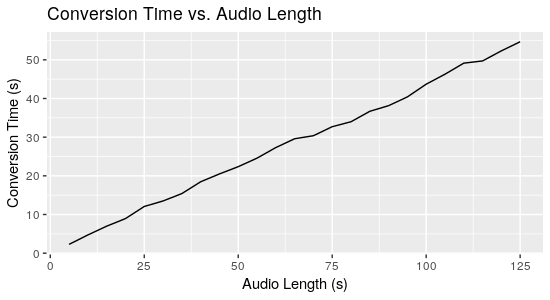
\includegraphics[width=\columnwidth]{img/conversion_time_from_audio_length}\newline
\caption{Audio-to-text conversion time based on audio length, using best trained DeepSpeech model.}
\label{fig:convtime-length}
\end{figure}

As a result, we use a smarter method: efficient and on-demand synchronization with search methods. At import time, we take a few minutes to calculate the average Words per Minute (WPM) of the audio. This is done by calculating the WPM of several hundred random samples from various portions of the audio, and averaging the rates together. We then calculate the expected position of a word using this WPM. This can be done bidirectionally:

\begin{flalign*}
&& \text{E(Word Position)} &= (pos_{audio} / 1000 / 60) * WPM && \\
&& \text{E(Audio Timestamp)} &= (pos_{text} / WPM) * 1000 * 60 && \\
\end{flalign*}

TODO: FIGURE FOR CLIP SEARCHING

We then take this expected position and do an expanding outwards search from it to match clips. A single clip (using the position we know) is taken from the original medium, which is then matched against clips in the new medium as we search. When the clips match, we've found our corresponding position. Three parameters are used here: clip size, clip movement, and match percentage. The clip size defines the size in words of the clips to search with. The clip movement defines how much this clip window should move after each iteration of the search. The match percentage determines how many words must match between the two clips.

\begin{figure}[ht]
TODO ALGORITHM
\newline
\caption{Search algorithm for synchronization.}
\label{alg:sync-algo}
\end{figure}

With a smaller clip size, we are comparing less words. Likewise, a larger clip size means we are comparing more words between the two mediums. The smaller the movement, the more accurate our position will be and the less likely we are to overshoot it; similarly, the larger the movement, the faster the comparisons but we are more likely to overshoot the actual position match. With a smaller match percentage, we are accepting a bit less accuracy for a faster search, and in doing this we can account for model inaccuracies as audio clips will never have a 100\% accurate conversion to text. With a larger match percentage, we will get a more accurate and confident answer, but we are likely to miss the match entirely due to being too strict in our matching.

\subsection{Optimization Methods}
TODO: FIGURES FOR EACH OF THESE
\subsubsection{Unidirectional Search}
\subsubsection{Cutoffs}
\subsubsection{Caching}
(BOTH AUDIO CONVERSIONS TO TEXT, AND POSITIONAL MATCHES WHICH CAN SERVE AS CUTOFFS AGAIN)
\subsubsection{Specialized Models}
\subsubsection{System Resources}

\section{Results}
\subsection{Model Accuracy}
\subsection{Engine Accuracy and Confidence}
\subsection{Optimal Engine Parameters}
\subsection{Synchronization Time}
\subsection{Overall Performance}
\subsection{Platform}

\section{Conclusion}
What have you learned?

Suggest future ideas.\\

List and number all bibliographical references at the end of your paper. When referenced in the text,
enclose the citation number in square brackets, for
example~\cite{Alpher04}.

{\small
\bibliographystyle{ieee}
\bibliography{egbib}
}

\end{document}
